\documentclass[11pt]{article}
\usepackage[margin=1in]{geometry}
\usepackage{amsmath,amssymb,amsthm}
\usepackage{mathtools}
\usepackage[numbers,square]{natbib}
\usepackage{booktabs}
\usepackage{tikz}
\usetikzlibrary{fit}
\usepackage{hyperref}
\hypersetup{hypertexnames=false}
\usepackage{cleveref}

% Theorem environments
\theoremstyle{definition}
\newtheorem{definition}{Definition}[section]
\theoremstyle{plain}
\newtheorem{theorem}{Theorem}[section]
\newtheorem{proposition}[theorem]{Proposition}
\newtheorem{corollary}[theorem]{Corollary}
\newtheorem{lemma}[theorem]{Lemma}
\theoremstyle{remark}
\newtheorem{remark}{Remark}[section]
\newtheorem{example}{Example}[section]

\newcommand{\enc}{\mathrm{enc}}
\newcommand{\dec}{\mathrm{dec}}
\newcommand{\fhat}{\hat{f}}
\newcommand{\cipher}[1]{\mathsf{C}(#1)}
\newcommand{\cipherS}[2]{\mathsf{C}_{#2}(#1)}
\newcommand{\orbitF}{\mathrm{orbit}_F}
\newcommand{\B}{\{0,1\}}

\title{Realizing Cipher Programs:\\Cut-Point Decomposition and Control-Flow Obliviousness}
\author{Alexander Towell\\\texttt{lex@metafunctor.com}}
\date{2026 (draft)}

\begin{document}
\maketitle

\begin{abstract}
A cipher map is a total function on bit strings that an untrusted
machine evaluates blindly; only a trusted machine holding the secret
can encode inputs and decode outputs.
The algebra of cipher \emph{types} and the confidentiality of single
maps and their compositions are developed
elsewhere~\cite{towell2026algebraic,towell2026cipher}.
This paper takes up the operational question those leave open: given an
ordinary program, how is it realized as a composition of cipher maps
the untrusted machine can run, and what does the realization leak?
We organize the paper around the difficulties this question raises.
Ciphering is \emph{infectious}: a cut at one node forces every node
that consumes its output, and every sibling input, to be ciphered as
well, so the ciphered region is upward-closed and a single cut can
cipher an entire single-rooted program.
Control flow forces a choice with no free option: branching on a cipher
Boolean is untrusted dispatch on a sum type, so a conditional must
either expose which branch ran (cheap, but leaks the test) or hide it
behind an oblivious multiplexer (which evaluates both branches); there
is no oblivious short-circuit.
Unbounded data-dependent control cannot be made oblivious at all, and
there the execution trajectory leaks.
We give the structural laws a realization must obey, a cost model for
the choices, and a tracing-based rewriter for the fragment where the
choices have clean defaults.
We do not claim a general compiler: the contribution is a calculus of
what is forced, what is chosen, and what each choice costs.

\medskip
\noindent\emph{Status: working draft. The technical core
(\Cref{sec:realizing}) was extracted from the algebraic-cipher-types
paper, where it was a distraction from the type-level results; it is
the natural home for the program-realization material and is being
developed into a standalone paper.}
\end{abstract}


%% ====================================================================
\section{Introduction}
\label{sec:intro}
%% ====================================================================

Trapdoor computing evaluates functions on data hidden behind a one-way
trapdoor.
A trusted machine encodes plaintext values into opaque cipher values and
hands them, together with cipher maps (total functions on bit strings),
to an untrusted machine that evaluates the maps blindly and returns
results it cannot decode~\cite{towell2026cipher}.
Two companion lines develop the pieces this paper composes: the
construction and confidentiality of a single cipher map (its four
properties, batch construction, and $\delta$-bounded
leakage)~\cite{towell2026cipher}, and the algebra of cipher
\emph{types}---products, sums, exponentials---together with the
orbit-closure confidentiality bound and the typed-composition
discipline~\cite{towell2026algebraic}.

This paper asks the operational question both leave open: \emph{given a
program, how is it realized as a composition of cipher maps, and what
does the realization leak?}
The naive hope---annotate a few functions and let a compiler do the
rest---meets a sequence of difficulties, and the paper is organized
around them.

\begin{enumerate}
\item \textbf{Ciphering propagates upward.}
  A cipher map's output is opaque, so any ancestor that consumes it must
  itself be a cipher map, and a cipher map's sibling inputs must be
  ciphered too.
  The ciphered region is upward-closed along data-flow edges; in a
  single-rooted program a single cut can cipher the entire tree
  (\Cref{sec:cipher-programs}).

\item \textbf{Control flow forces a choice.}
  Branching on a cipher Boolean is untrusted dispatch on the sum
  $\mathbf{1}+\mathbf{1}$, which the sum-type
  impossibility~\cite{towell2026algebraic} forbids without leaking the
  test.
  A conditional must either expose which branch ran (cheap, but leaks)
  or hide it behind an oblivious multiplexer (which evaluates both
  branches).
  There is no oblivious short-circuit (\Cref{sec:branching}).

\item \textbf{Some control flow cannot be made oblivious at all.}
  Bounded conditionals unroll to a fixed computation graph; unbounded
  data-dependent control (loops, recursion, data-dependent indexing)
  cannot, and there the execution trajectory leaks---the
  cipher-Turing-machine regime (\Cref{sec:branching}).

\item \textbf{Cost.}
  Oblivious selection over a result type $R$ costs $O(|R|^2)$; fusing a
  region into one cipher map costs $O(|X|)$ over its input domain.
  Where to cut is a multi-dimensional optimization over space, build
  time, and leakage (\Cref{sec:tm-vs-tree}).

\item \textbf{A decision space, not a default.}
  Each node carries choices: cipher or leave plain, expose or hide a
  branch, fuse or compose, joint or component-wise encode its inputs.
  A practical rewriter must surface these as annotations with sensible
  defaults (\Cref{sec:auto}).
\end{enumerate}

We make these precise and give the structural laws a realization must
obey (\Cref{sec:realizing}), then sketch a tracing-based rewriter and
its decision space (\Cref{sec:auto}).


%% ====================================================================
\section{Background}
\label{sec:background}
%% ====================================================================

We take the cipher map abstraction and its four properties (totality,
representation uniformity $\delta$, correctness $\eta$, composability)
from~\cite{towell2026cipher}, and the construction of a cipher map for a
given function over a finite domain from its batch (perfect-hash)
construction~\cite[Sec.~6]{towell2026cipher}.
We write $\cipher{X}$ for the cipher type of a latent type $X$ (the set
of valid encodings), $\fhat$ for a cipher map, and $\orbitF(c)$ for the
orbit closure of a cipher value $c$ under an operation set $F$.
From the algebraic-cipher-types paper~\cite{towell2026algebraic} we take
the type-constructor trade-offs (products leak correlations, sums force
the tag-versus-pattern-match impossibility, exponentials are cipher maps
themselves), the orbit-closure confidentiality bound
$H(X \mid \mathcal{V}_F(c)) \geq H(X) - \log_2|\orbitF(c)|$, and the
typed-composition discipline that bounds orbit growth at construction
time.
This paper builds programs out of those constructed maps; it does not
re-derive construction or the type-level results.

%% ====================================================================
\section{Programs as Cipher-Map Compositions}
\label{sec:realizing}
%% ====================================================================

The type-theoretic results of the cipher-type algebra and orbit-closure framework~\cite{towell2026algebraic} bound what any
cipher-program realization can achieve.
A cipher program is a composition of cipher maps and plain operations
over opaque bit strings: the untrusted machine evaluates the cipher
maps blindly and plumbs their cipher-valued outputs through ordinary
code.
The atomic primitive is the construction of a single cipher map from a
function over a chosen domain; a program is built by composing such
maps by hand, deciding where each one sits.
Because a cipher map is just a total function on bit strings, it is a
portable artifact: it composes by ordinary function composition, in
any language or at a shell, with no special runtime.
This section describes the structure of such hand-built programs---where
cipher maps must go, and what each placement leaks.
Automating this construction---rewriting an arbitrary annotated
program into a cipher program (combiner synthesis, control-flow
obliviousness, a per-node and per-argument decision space)---is the
problem this paper takes up; \Cref{sec:auto} sketches the rewriter and
its decision space.


%% --------------------------------------------------------------------
\subsection{Expression-Tree Decomposition}
\label{sec:cipher-programs}
%% --------------------------------------------------------------------

The type-theoretic trade-offs of the product and sum trade-offs~\cite{towell2026algebraic} have a
direct operational realization: given a program represented as an
expression tree, which subtrees should be replaced by cipher maps?

\begin{definition}[Cipher node and cut-point placement]
\label{def:cipher-node}
A \emph{cipher node} in a program's expression tree is a node realized
as a cipher map: the function computed by that node and its subtree,
restricted to a chosen domain, is evaluated at construction time on the
trusted machine and stored as a cipher map backed by a perfect hash
function~\cite{fredman1984storing}.
A \emph{cut-point placement} is a choice of which nodes are cipher
nodes; the cipher maps lying above the lowest cipher nodes form a
\emph{combiner} that consumes their cipher-valued outputs.
The programmer makes this choice by hand; \Cref{rem:cipher-propagation}
constrains it.
\end{definition}

The placement of cipher node annotations controls the encoding
granularity:

\begin{itemize}
\item \textbf{Annotation at the root}: the entire program is one cipher
  map.  Maximum confidentiality (no intermediate values exposed), maximum
  space ($O(|X|)$ where $X$ is the input domain of the full program).
\item \textbf{Annotation at the leaves}: each leaf function is a
  separate cipher map.  The combiner chains them.  Intermediate cipher
  values are visible to the untrusted machine, leaking correlations
  between components (as in the product-type trade-off of
  the product trade-off~\cite{towell2026algebraic}).
\item \textbf{Annotation at intermediate nodes}: a spectrum between the
  two extremes.  Deeper annotations absorb more computation into cipher
  maps (more confidential, more space); shallower annotations expose
  more structure (less space, more leakage).
\end{itemize}

\begin{remark}[Ciphering propagates upward through the tree]
\label{rem:cipher-propagation}
Cut-point placement is not free leaf-by-leaf.
Replacing a subtree with a cipher map makes its output a cipher value,
and any ancestor that \emph{semantically consumes} that value must then
be a cipher map too, since the untrusted machine cannot decode it; and
because a cipher map takes cipher inputs, its \emph{sibling} inputs must
be cipher values as well.
For ordinary data operations there is no choice: an arithmetic node or a
comparison fed a cipher value can only proceed as a cipher map.
The ciphered region is thus upward-closed along data-flow edges, with
the cut points as its lower frontier (the combiner of
\Cref{def:cipher-node} is exactly this region); only pure
plumbing---moving, pairing, or returning a cipher value untouched---may
remain plaintext.
Because every value in a single-rooted expression tree meets at the
root, a single cut whose result reaches the output through data
operations ciphers the entire tree (\Cref{fig:cipher-tree}).
Control flow is the one place a genuine choice appears, developed in
\Cref{sec:branching}: branching on a cipher Boolean either exposes which
branch was taken---the cheap default, which leaks the test---or hides it
behind an oblivious multiplexer, which forces both branches to be
ciphered and evaluated.
\Cref{fig:cipher-tree} shows the hiding choice.
\end{remark}

\begin{figure}[t]
\centering
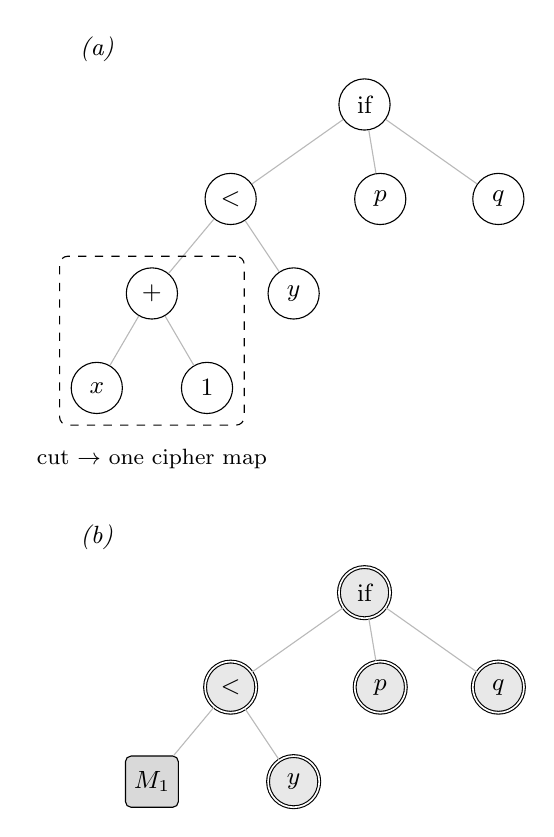
\begin{tikzpicture}[
  plain/.style={circle, draw, minimum size=6.5mm, inner sep=0pt, font=\small},
  ciph/.style={circle, draw, double, double distance=0.6pt, fill=gray!18,
               minimum size=6.5mm, inner sep=0pt, font=\small},
  cmap/.style={rectangle, rounded corners=2pt, draw, fill=gray!30,
               minimum height=6.5mm, inner sep=3pt, font=\small},
  lk/.style={-, gray!55}]

%% Panel (a): plaintext tree for  if ((x+1) < y) then p else q
\node[font=\itshape\small] at (-3.4,0.7) {(a)};
\node[plain] (if)  at (0,0)      {if};
\node[plain] (lt)  at (-1.7,-1.2){$<$};
\node[plain] (p)   at (0.2,-1.2) {$p$};
\node[plain] (q)   at (1.7,-1.2) {$q$};
\node[plain] (pl)  at (-2.7,-2.4){$+$};
\node[plain] (y)   at (-0.9,-2.4){$y$};
\node[plain] (x)   at (-3.4,-3.6){$x$};
\node[plain] (one) at (-2.0,-3.6){$1$};
\draw[lk] (if)--(lt); \draw[lk] (if)--(p); \draw[lk] (if)--(q);
\draw[lk] (lt)--(pl); \draw[lk] (lt)--(y);
\draw[lk] (pl)--(x);  \draw[lk] (pl)--(one);
\node[draw, dashed, rounded corners=3pt, inner sep=4pt,
      fit=(pl)(x)(one)] (cut) {};
\node[font=\footnotesize] at (-2.7,-4.5) {cut $\to$ one cipher map};

%% Panel (b): after the cut, percolated to the root
\begin{scope}[yshift=-6.2cm]
\node[font=\itshape\small] at (-3.4,0.7) {(b)};
\node[ciph] (if2) at (0,0)      {if};
\node[ciph] (lt2) at (-1.7,-1.2){$<$};
\node[ciph] (p2)  at (0.2,-1.2) {$p$};
\node[ciph] (q2)  at (1.7,-1.2) {$q$};
\node[cmap] (m1)  at (-2.7,-2.4){$M_1$};
\node[ciph] (y2)  at (-0.9,-2.4){$y$};
\draw[lk] (if2)--(lt2); \draw[lk] (if2)--(p2); \draw[lk] (if2)--(q2);
\draw[lk] (lt2)--(m1);  \draw[lk] (lt2)--(y2);
\end{scope}
\end{tikzpicture}
\caption{Ciphering propagates up an expression tree, here for
\texttt{if ($x+1 < y$) then $p$ else $q$}.
(a)~The plaintext tree; cutting at $+$ rolls the subtree $x+1$ into a
single cipher map.
(b)~The cut subtree is now one opaque cipher map $M_1$ (rounded box);
its cipher output forces $<$ into a cipher comparison, which pulls in
the sibling $y$.
The cipher Boolean then reaches \texttt{if}, where a choice appears: the
cheap default \emph{exposes} which branch was taken (leaking the test),
while \emph{hiding} it---the case drawn here---turns \texttt{if} into a
cipher multiplexer that pulls in both branches $p$ and $q$, ciphering the
entire tree above the cut (\Cref{sec:branching}).
Double-circled shaded nodes are cipher nodes.}
\label{fig:cipher-tree}
\end{figure}

\begin{remark}[Shared variables and compositional leakage]
\label{rem:shared-vars}
When two cipher nodes $f$ and $g$ share an input variable $x$, the
untrusted machine observes two cipher values $\enc_f(x, k_f)$ and
$\enc_g(x, k_g)$ derived from the same latent $x$.
Even if both encodings are individually $\delta$-close to uniform, the
joint distribution of $(\enc_f(x), \enc_g(x))$ preserves the correlation
(as in \cite[Prop.~8.1]{towell2026cipher}).
The only mitigation is to merge $f$ and $g$ into a single cipher node
(eliminating the shared intermediate) or to inject noise queries that
dilute the correlation signal.
\end{remark}

\paragraph{Manual composition.}
In this paper cipher programs are built by hand: one constructs each
cipher map with the primitive of \Cref{def:cipher-node} and wires its
cipher-valued output into the input of the next, exactly as one composes
ordinary functions.
Because cipher maps are portable total functions on bit strings, the
composition needs no special runtime---it runs in plain Python, or as
chained command-line tools, or in any language that can hash and look
up.
Hand composition is enough for everything we use: the cipher Boolean
algebra and Boolean search of the cipher Boolean algebra~\cite{towell2026algebraic}, the typed chains
of typed composition chains~\cite{towell2026algebraic}, and the partial-filtering retrieval of
partial filtering~\cite{towell2026algebraic}.
It also keeps the placement of every cut point, and every
expose-versus-hide decision (\Cref{sec:branching}), under explicit
control, which is what lets the constructions below exploit structure
that a mechanical rewrite would miss.
Recovering the composition automatically from an annotated source
program---tracing which nodes are cipher nodes, synthesizing the
combiner, and discharging the control-flow choices---is a separate
undertaking with its own decision space, developed in a companion
paper.


%% --------------------------------------------------------------------
\subsection{Branching and the Limits of Oblivious Control}
\label{sec:branching}
%% --------------------------------------------------------------------

Control flow is where the realization meets its limits, and the
boundary is exactly the sum-type impossibility of
the sum-type analysis~\cite{towell2026algebraic}.
A conditional \texttt{if $e$ then $P$ else $Q$} over a cipher Boolean
$e$ becomes a cipher multiplexer
$\mathrm{ite} : \cipher{\mathbf{2}} \times \cipher{R} \times \cipher{R}
\to \cipher{R}$, $\mathrm{ite}(t, a, b) = a$ if $t$ else $b$, where
$\mathbf{2} = \mathbf{1}+\mathbf{1}$ is the Boolean type.
The untrusted machine evaluates $\mathrm{ite}$ blindly and never learns
$t$; the cost is hidden in its \emph{inputs}, since materializing both
$\cipher{R}$ arguments means evaluating both branches.

\begin{proposition}[No oblivious short-circuit]
\label{prop:no-short-circuit}
Evaluate \texttt{if $e$ then $P$ else $Q$} on the untrusted machine over
a cipher Boolean $e = \enc(t,k)$, producing a cipher value of the result
type.
If the untrusted machine evaluates only the branch selected by $t$, then
it has performed untrusted pattern matching on $\mathbf{1}+\mathbf{1}$
and, by the sum-type impossibility~\cite{towell2026algebraic}, leaks $t$ with advantage at least
$1-\delta$.
Hiding $t$ therefore forbids short-circuiting: the untaken branch's
contribution cannot be skipped.
It is paid instead either at evaluation time---evaluate both branches and
combine them through $\mathrm{ite}$---or at construction time, by a fused
eliminator over the joint domain (the oblivious-elimination routes~\cite{towell2026algebraic}).
\end{proposition}

\begin{proof}
Evaluating only the selected branch makes the untrusted machine's action
(run $P$ versus run $Q$) a function $s(\enc(v,k))$ that equals $t$ on
valid encodings; this is the selector of the sum-type impossibility~\cite{towell2026algebraic},
a tag distinguisher, so $t$ leaks.
Hiding $t$ requires the untrusted machine's run-time behavior to be
independent of $t$, so it cannot run one branch in place of the other.
Two $t$-independent behaviors still compute the result: evaluate both
branches and apply $\mathrm{ite}$ (which selects via a cipher map without
exposing $t$), or evaluate a single fused cipher map for the whole
conditional whose construction already ranged over both branches.
In either case the untaken branch is evaluated---at run time or at
construction time---never skipped.
\end{proof}

The plaintext efficiency of \texttt{if}---run only the taken branch---is
therefore precisely what cannot be done obliviously.
Three regimes follow, by how the branches scale.

\emph{Bounded, fixed-shape branches.}
When $P$ and $Q$ are straight-line (or themselves bounded conditionals),
the untrusted machine performs a \emph{fixed}, data-independent set of
operations: it evaluates every branch and muxes.
Confidentiality is free; the cost is that $k$ nested conditionals
evaluate all $2^k$ leaves.
\Cref{fig:cipher-tree} is the single-conditional case.

\emph{Total-but-partial branches.}
Evaluating the untaken branch is safe even when it would be undefined in
plaintext---\texttt{if $x \neq 0$ then $y/x$ else $0$} evaluates $y/x$ at
$x=0$---because cipher maps are total: the spurious evaluation returns a
noise value (the noise-unreliability property~\cite{towell2026algebraic}) that the multiplexer
discards.
Totality (Property~1) is what makes both-branches evaluation correct.

\emph{Unbounded, data-dependent control.}
When the number of operations depends on a cipher value---a loop
\texttt{while $c$ do $\ldots$} or a recursion whose depth is data
dependent---the operation set can no longer be fixed.
Two options remain: unroll to a \emph{public} bound $N$ and obliviously
mask the iterations past the true count (cost $O(N)$ regardless of the
data, tag hidden), or test the cipher condition each step to decide
whether to continue, which is untrusted dispatch per step and leaks the
trajectory (the trip count, a function of the data).
There is no oblivious unrolling without a public bound.

These regimes are one statement about \emph{shape}: the expression-tree
realization is oblivious exactly because it compiles to a fixed,
data-independent computation graph.
Branching is the atomic data-dependent decision, handled obliviously
only by evaluating both sides; unbounded data-dependent control cannot
be flattened to a fixed graph, and there the trajectory must leak.
That unbounded case is a cipher Turing machine, whose per-step
$(\text{state}, \text{direction})$ leakage is the loop leak above; it is
why this paper takes the fixed-graph expression tree, not the Turing
machine, as the realization (cf.\ \Cref{sec:tm-vs-tree}).

\begin{remark}[The multiplexer is not free]
\label{rem:mux-cost}
As a cipher map, $\mathrm{ite} : \cipher{\mathbf 2} \times \cipher{R}
\times \cipher{R} \to \cipher{R}$ has domain $2|R|^2$, so oblivious
selection over a result type $R$ costs $O(|R|^2)$ space---the
product-encoding cost of the product trade-off~\cite{towell2026algebraic} resurfacing inside
control flow.
Fusing the whole conditional into one cipher map over the input domain
$X$ costs $O(|X|)$ instead; which is cheaper is the granularity choice of
\Cref{sec:cipher-programs}.
And if $P$ and $Q$ return different variants, $\mathrm{ite}$'s output is
a cipher sum, and the dispatch obligation of the sum-type impossibility~\cite{towell2026algebraic}
reappears at the next consumer rather than dissolving.
\end{remark}


%% --------------------------------------------------------------------
\subsection{Cut-Point Structure}
\label{sec:tm-vs-tree}
%% --------------------------------------------------------------------

\begin{definition}[Cut point]
\label{def:cut-point}
Given a plaintext computation $P$ represented as a directed acyclic
graph with functions at nodes and data flow along edges, a \emph{cut
point} is a node whose subgraph of ancestors is replaced, during
construction, by a single cipher map.
Edges entering the cut point carry plaintext on the trusted machine
and cipher values on the untrusted machine; edges leaving the cut
point carry cipher values throughout.
A \emph{cut-point set} is a collection of cut points such that every
input of $P$ reaches at least one of them; the cipher maps at the cut
points together with the unmarked nodes above them (which evaluate as
plain code on the cipher bytes) compute $P$ on the untrusted machine.
\end{definition}

\paragraph{What leaks above the cut points.}
Exactly what remains plaintext above the cut points is the leakage
profile: the collection of intermediate cipher values flowing between
cipher nodes, plus whatever the unmarked plain operations reveal about
those values (equality checks, branching, dictionary lookups).
Multiple cut points sharing a latent input leak that input's
correlation structure across their outputs, per the product-encoding
trade-off (the product trade-off~\cite{towell2026algebraic}).

\paragraph{What bounds the orbit.}
A typed-chain decomposition (distinct cipher spaces between
consecutive cut points) inherits the bound $\sum_i N_i$ of
the typed-chain orbit bound~\cite{towell2026algebraic}; for a depth-$k$ tree with binary combinators
starting from $m$ distinct latent inputs, the bound is
$\sum_{i=0}^{k} m^{2^i}$.
Decompositions that reuse a single cipher space across cut points
(equivalently, that admit a self-loop in the cipher-map dependency
graph) fall outside the typed-chain hypothesis and require a separate
argument; for deterministic iterated computations of length $T$, a
single-trajectory bound of $T+1$ orbit elements per starting cipher
value is straightforward but the leakage profile is severe:
every per-step plaintext signal needed to advance the loop (selectors,
indices, halting time) is observable.
This is the unbounded-control regime of \Cref{sec:branching}: a
self-loop is exactly the data-dependent control that cannot be flattened
to a fixed graph.

\begin{example}[Regex matching as a typed cut-point chain]
\label{ex:regex-cut-points}
Consider matching a fixed regular expression $R$ of size $r$ against a
string $x \in \Sigma^\ell$, with DFA state set $Q_R$ (in the worst
case $|Q_R| = 2^{O(r)}$ via subset construction; for many regexes
much smaller).
The natural typed-chain decomposition places $\ell$ cut points
$\hat{\tau}_0, \ldots, \hat{\tau}_{\ell-1}$ with $\hat{\tau}_i :
\cipher{Q_R}_i \times \cipher{\Sigma} \to \cipher{Q_R}_{i+1}$, each
of space $O(|Q_R| \cdot |\Sigma|)$, total
$O(\ell \cdot |Q_R| \cdot |\Sigma|)$.
The orbit is bounded by $1 + \ell$ from the typed-chain orbit bound~\cite{towell2026algebraic}
(single state value at each level), and the leakage above the cut
points is the $(\ell + 1)$-tuple of intermediate cipher state values
$c_0, \ldots, c_\ell$.
The same computation can be expressed as a self-loop on a single
cipher space $\cipher{Q_R \times \Sigma}$ with a single transition
cipher map of space $O(|Q_R|^2 \cdot |\Sigma|)$ (constant in $\ell$),
but the leakage then includes a plaintext (next-state-selector,
direction) pair per step, redacting only the tape contents.
The choice between the typed chain and the self-loop is therefore not
about space (the typed chain is asymptotically smaller per cut point
once $\ell > |Q_R|$) but about \emph{which structure leaks}.
\end{example}



%% ====================================================================
\section{Automatic Rewriting and the Decision Space}
\label{sec:auto}
%% ====================================================================

\Cref{sec:realizing} described hand construction.
We now sketch how to recover a cipher program from an annotated source
program, and why the recovery is a space of decisions rather than a
single default.

\paragraph{Tracing.}
A practical rewriter marks chosen functions with a \texttt{@cipher\_node}
decorator and runs a tracing pass over the declared input domain.
The trace records which cipher nodes are called, with what arguments,
and what they return.
From the trace the rewriter (i)~builds a cipher map for each traced
node, (ii)~builds the combiner cipher maps for the nodes above the cut
frontier, over the tuples of component cipher outputs, and (iii)~infers
which program inputs feed which node from the observed call pattern.
By \Cref{rem:cipher-propagation} the combiner is forced: every node
above a cut that consumes a cipher value is itself a cipher map.

\paragraph{The decision space.}
The trace does not determine the realization; several independent
choices remain at each node, and a usable annotation system must expose
them with defaults:
\begin{itemize}
\item \emph{Cut depth} (fuse vs.\ compose): absorb a subtree into one
  cipher map (smaller orbit, no intermediates exposed, $O(|X|)$ space)
  or keep components separate (smaller maps, intermediates exposed).
\item \emph{Branch policy} (expose vs.\ hide): leak the test and
  short-circuit, or hide it behind a multiplexer and evaluate both
  branches (\Cref{sec:branching}).
\item \emph{Input granularity} (joint vs.\ component-wise): encode a
  node's arguments together (hides their correlation, costs the product
  domain) or separately (exposes correlation, cheaper).
\end{itemize}
Each choice trades confidentiality, space, build time, and evaluation
cost against one another; the orbit bound and the cost model of
\Cref{sec:tm-vs-tree} score them, but selecting the cut-point set that
minimizes leakage subject to a space budget is an open optimization
(\Cref{sec:open}).

\paragraph{Reference implementation.}
A Python implementation (\texttt{cipher-maps}) realizes the tracing
rewriter for the straight-line and bounded-conditional fragment, backing
each cipher node with a perfect hash function~\cite{fredman1984storing}.
Short-circuit conditionals are handled by evaluating all branches and
combining obliviously, as \Cref{sec:branching} requires.
Unbounded data-dependent control is rejected (or requires a
user-supplied bound), per the trajectory-leakage limit.


%% ====================================================================
\section{Open Problems}
\label{sec:open}
%% ====================================================================

\begin{enumerate}
\item \emph{Cut-point optimization.}
  Formulate cut-point selection as a constrained optimization: minimize
  total leakage (summed orbit log-sizes) subject to a construction-space
  budget, over the choices of \Cref{sec:auto}.
  Is it tractable, or NP-hard like related partitioning problems?

\item \emph{Plain operations on cipher bytes.}
  Above the cut points, some operations need not be cipher maps---they
  may run as plain code on the cipher bytes (equality tests, dictionary
  lookups, moves).
  Each leaks something specific (equality reveals collisions; lookups
  reveal bucket membership).
  Characterize this leakage and when plain operations are preferable to
  a precomputed combiner.

\item \emph{Bounded oblivious control without a public bound.}
  Loops with a data-dependent trip count leak the count unless unrolled
  to a public bound.
  Are there constructions that bound the leakage to coarse information
  (e.g.\ the order of magnitude of the count) at sub-linear overhead,
  short of full ORAM?

\item \emph{Verified obliviousness.}
  Given an annotated program, statically certify that the realized
  cipher program leaks only the declared signals (the branch exposures
  and trajectory observables), and nothing more.
\end{enumerate}


\bibliographystyle{plainnat}
\bibliography{references}

\end{document}
